\let\negmedspace\undefined
\let\negthickspace\undefined
\documentclass[journal,12pt,onecolumn]{IEEEtran}
\usepackage{cite}
\usepackage{amsmath,amssymb,amsfonts,amsthm}
\usepackage{algorithmic}
\usepackage{graphicx}
\usepackage{textcomp}
\usepackage{xcolor}
\usepackage{txfonts}
\usepackage{listings}
\usepackage{enumitem}
\usepackage{mathtools}
\usepackage{gensymb}
\usepackage{comment}
\usepackage[breaklinks=true]{hyperref}
\usepackage{tkz-euclide}
\usepackage{listings}
\usepackage{gvv}
\def\inputGnumericTable{}
\usepackage[latin1]{inputenc}
\usepackage{color}
\usepackage{array}
\usepackage{longtable}
\usepackage{calc}
\usepackage{multirow}
\usepackage{hhline}
\usepackage{ifthen}
\usepackage{lscape}

\newtheorem{theorem}{Theorem}[section]
\newtheorem{problem}{Problem}
\newtheorem{proposition}{Proposition}[section]
\newtheorem{lemma}{Lemma}[section]
\newtheorem{corollary}[theorem]{Corollary}
\newtheorem{example}{Example}[section]
\newtheorem{definition}[problem]{Definition}
\newcommand{\BEQA}{\begin{eqnarray}}
\newcommand{\EEQA}{\end{eqnarray}}
\newcommand{\define}{\stackrel{\triangle}{=}}
\theoremstyle{remark}
\newtheorem{rem}{Remark}
\begin{document}

\bibliographystyle{IEEEtran}
\vspace{3cm}

\title{NCERT Discrete - 11.9.1.2}
\author{EE23BTECH11049 - Praful Kesavadas$^{*}$% <-this % stops a space
}
\maketitle

\bigskip

\renewcommand{\thefigure}{\theenumi}
\renewcommand{\thetable}{\theenumi}

\textbf{Question : 11.9.1.2:}\\
Write the first five terms of the sequence whose $n^{th}$ terms  $x\brak{n} = \frac{n}{n+1}$\\
\solution\\
\begin{table}[ht]
\centering
\begin{tabular}{|c|c|c|}
    \hline
    \textbf{Term} & \textbf{Value} & \textbf{Description}\\
    \hline
    $x(0)$ & - & First term\\
    \hline
    $d$ & - & Common Difference\\
    \hline
    $x(n-1)$ & $x(0)+(n-1)d$ & General term\\
    \hline
    $x(p-1)$ & $a$ & pth term\\
    \hline
    $x(q-1)$ & $b$ & qth term\\
    \hline
    $x(r-1)$ & $c$ & rth term\\
    \hline
  \end{tabular}
  

\caption{Input Parameters}
\end{table}
Here, Z-transform
\begin{align}
X(z) &= \sum_{i=-\infty}^\infty\ x\brak{n}.z^{-n}\\
&= \sum_{i=-\infty}^\infty \frac{n}{n+1}.u(n). z^{-n}\\
&= \sum_{i=-\infty}^\infty u\brak{n}.z^{-n} - \frac{1}{n+1} u\brak{n}.z^{-n}
\end{align}
Now, 
\begin{align}
u\brak{n} &\xleftrightarrow Z  \frac{1}{1-z^{-1}}, \quad{|z|>1}\\
\frac{-1}{n+1}.u\brak{n} &\xleftrightarrow Z  z\log(1-z^{-1}), \quad{|z|>1}\\
X(z) &= \frac{1}{1-z^{-1}} + z\log{(1-z^{-1})} ,\quad{|z|>1}
\end{align}
\begin{figure}[ht!]
    \centering
    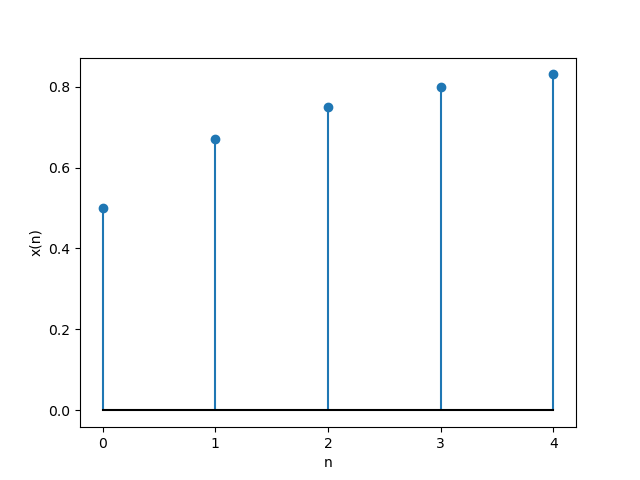
\includegraphics[width=\columnwidth]{figs/graph1.png}
    \caption{Stem plot for x(n)}
    \label{fig:11.9.1.2fig1}
\end{figure}
\end{document}
